\documentclass[lettersize,journal]{IEEEtran}

\usepackage{amsmath,amssymb,amsfonts}
\usepackage{graphicx}
\usepackage{booktabs}
\usepackage{array}
\usepackage{stfloats}
\usepackage{url}
\usepackage{cite}

\graphicspath{{figures/}}

\newcommand{\permcontrol}{\textsc{Perm}}
\newcommand{\polcontrol}{\textsc{Rand}}

\renewcommand{\thesection}{S\arabic{section}}
\renewcommand{\thetable}{S\arabic{table}}
\renewcommand{\thefigure}{S\arabic{figure}}

\begin{document}

\title{Supplementary Material for\\
``Does the Score Do the Work? Permutation Controls for\\
Score-Weighted Metaheuristics''}

\author{}
\markboth{Supplementary Material}{}
\maketitle

\section{Displacement Induced by the Weighting}
\label{sec:supp:magnitude}

Fig.~\ref{fig:supp:magnitude} reports the normalised displacement $\rho$ of
the main text for every graph configuration used in the original report and
in its reference implementation. It is the precondition check the main text
summarises: a permutation control is informative only where the mechanism it
neutralises is active.

\begin{figure}[t]
\centering
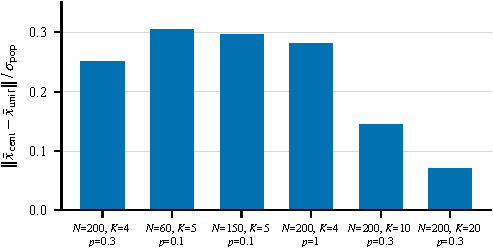
\includegraphics{fig_mechanism_magnitude}
\caption{Displacement induced by centrality weighting, in units of the
population's own spread. Across the published and implemented settings the
mechanism moves each update by a quarter to a third of the population spread;
on the vertex-transitive ring lattice ($p=0$) it is inert to machine
precision.}
\label{fig:supp:magnitude}
\end{figure}

\section{Per-Function Results on CEC2017}
\label{sec:supp:tables}

Table~\ref{tab:cec30} gives the median error of every arm on every
function of the suite at $D=30$, from which the suite-level summaries in the
main text are computed. Bold marks the best arm and any arm not distinguishable
from it by a paired Wilcoxon test at $\alpha=0.05$.

\begin{table*}[t]
\caption{Median error on CEC2017 at $D=30$ over 30 runs, budget $10^{4}D$. Bold marks the best arm and any arm not distinguishable from it by a paired Wilcoxon test at $\alpha=0.05$. The last row gives mean Friedman ranks over the suite.}
\label{tab:cec30}
\centering
\small
\setlength{\tabcolsep}{4pt}
\begin{tabular}{@{}llrrrrrr@{}}
\toprule
F & Class & \textsc{Social} & \permcontrol{} & \textsc{Unif}$_4$ & \textsc{Fix}$_{16}$ & \polcontrol{} & \textsc{Ads} \\
\midrule
$F_{1}$ & Unimodal & \textbf{1.05e+03} & \textbf{1.98e+03} & \textbf{1.72e+03} & 2.62e+03 & \textbf{2.05e+03} & \textbf{1.60e+03} \\
$F_{3}$ &  & \textbf{7.11e+01} & \textbf{8.01e+01} & \textbf{7.62e+01} & \textbf{8.08e+01} & \textbf{7.43e+01} & \textbf{7.85e+01} \\
$F_{4}$ & Simple multimodal & \textbf{5.34e+02} & \textbf{5.62e+02} & \textbf{5.27e+02} & \textbf{5.58e+02} & 6.26e+02 & \textbf{5.50e+02} \\
$F_{5}$ &  & \textbf{3.22e-04} & \textbf{3.29e-04} & \textbf{3.10e-04} & \textbf{2.68e-04} & \textbf{4.40e-04} & \textbf{4.02e-04} \\
$F_{6}$ &  & \textbf{4.37e+02} & \textbf{4.09e+02} & \textbf{4.09e+02} & \textbf{3.84e+02} & \textbf{4.29e+02} & \textbf{4.56e+02} \\
$F_{7}$ &  & \textbf{3.90e+02} & \textbf{3.69e+02} & \textbf{3.81e+02} & \textbf{4.08e+02} & 4.24e+02 & 4.07e+02 \\
$F_{8}$ &  & \textbf{9.60e+00} & \textbf{9.24e+00} & \textbf{9.28e+00} & \textbf{1.07e+01} & \textbf{9.33e+00} & \textbf{9.83e+00} \\
$F_{9}$ &  & \textbf{3.85e+03} & \textbf{3.99e+03} & \textbf{3.95e+03} & \textbf{4.01e+03} & \textbf{4.25e+03} & \textbf{4.17e+03} \\
$F_{10}$ &  & \textbf{5.43e+04} & \textbf{5.21e+04} & \textbf{4.92e+04} & \textbf{5.11e+04} & 5.26e+04 & 5.09e+04 \\
$F_{11}$ & Hybrid & \textbf{3.37e+06} & \textbf{4.18e+06} & \textbf{4.53e+06} & \textbf{4.10e+06} & \textbf{4.60e+06} & 4.73e+06 \\
$F_{12}$ &  & 1.02e+05 & 1.06e+05 & 1.25e+05 & \textbf{9.61e+04} & 1.29e+05 & 1.14e+05 \\
$F_{13}$ &  & \textbf{1.08e+05} & \textbf{1.14e+05} & \textbf{1.03e+05} & \textbf{1.07e+05} & \textbf{1.04e+05} & \textbf{1.10e+05} \\
$F_{14}$ &  & 6.76e+04 & \textbf{6.84e+04} & 7.08e+04 & \textbf{6.39e+04} & 6.84e+04 & 6.83e+04 \\
$F_{15}$ &  & \textbf{4.40e+03} & \textbf{5.17e+03} & \textbf{3.88e+03} & 5.70e+03 & 5.23e+03 & 5.15e+03 \\
$F_{16}$ &  & \textbf{1.80e+03} & \textbf{1.63e+03} & \textbf{1.71e+03} & \textbf{1.86e+03} & \textbf{1.81e+03} & \textbf{1.69e+03} \\
$F_{17}$ &  & \textbf{1.75e+05} & \textbf{1.65e+05} & \textbf{1.52e+05} & \textbf{1.71e+05} & 2.10e+05 & 2.07e+05 \\
$F_{18}$ &  & \textbf{4.21e+04} & \textbf{3.97e+04} & \textbf{4.40e+04} & 5.28e+04 & 5.15e+04 & \textbf{5.06e+04} \\
$F_{19}$ &  & 2.09e+03 & \textbf{1.92e+03} & 2.12e+03 & \textbf{2.26e+03} & 2.30e+03 & 2.28e+03 \\
$F_{20}$ &  & \textbf{6.16e+02} & \textbf{7.09e+02} & 7.27e+02 & \textbf{7.93e+02} & \textbf{7.68e+02} & \textbf{6.36e+02} \\
$F_{21}$ & Composition & \textbf{1.71e+03} & \textbf{1.69e+03} & \textbf{2.03e+03} & 2.06e+03 & 2.01e+03 & 2.20e+03 \\
$F_{22}$ &  & \textbf{2.01e+02} & \textbf{2.01e+02} & 2.01e+02 & \textbf{2.05e+02} & 2.03e+02 & \textbf{2.02e+02} \\
$F_{23}$ &  & \textbf{2.00e+02} & \textbf{2.00e+02} & 2.01e+02 & 2.03e+02 & 2.02e+02 & 2.01e+02 \\
$F_{24}$ &  & \textbf{4.38e+02} & \textbf{4.43e+02} & \textbf{4.50e+02} & \textbf{4.45e+02} & 4.61e+02 & 4.54e+02 \\
$F_{25}$ &  & \textbf{7.95e+02} & \textbf{8.00e+02} & \textbf{8.00e+02} & \textbf{7.91e+02} & \textbf{7.98e+02} & \textbf{7.98e+02} \\
$F_{26}$ &  & \textbf{1.24e+03} & \textbf{1.40e+03} & \textbf{1.21e+03} & \textbf{1.34e+03} & \textbf{1.44e+03} & \textbf{1.34e+03} \\
$F_{27}$ &  & \textbf{9.68e+01} & \textbf{1.06e+02} & \textbf{9.29e+01} & \textbf{1.26e+02} & \textbf{1.31e+02} & \textbf{1.51e+02} \\
$F_{28}$ &  & \textbf{4.47e+04} & \textbf{5.20e+04} & \textbf{4.91e+04} & \textbf{5.15e+04} & \textbf{5.25e+04} & \textbf{5.19e+04} \\
$F_{29}$ &  & \textbf{8.48e+05} & \textbf{9.16e+05} & \textbf{8.80e+05} & \textbf{8.98e+05} & 9.77e+05 & 1.01e+06 \\
\midrule
\multicolumn{2}{@{}l}{Mean rank} & 3.121 & 3.170 & 3.335 & 3.676 & 3.977 & 3.720 \\
\bottomrule
\end{tabular}
\end{table*}


\section{Per-Function Effect Sizes}
\label{sec:supp:forest}

Fig.~\ref{fig:supp:forest} shows the effect of destroying the structure--weight
correspondence on each function separately, with bootstrap intervals, for every
suite and budget. The main text reports only the suite-level summaries of these
distributions. No interval excludes zero after Holm correction in any panel.

\begin{figure*}[t]
\centering
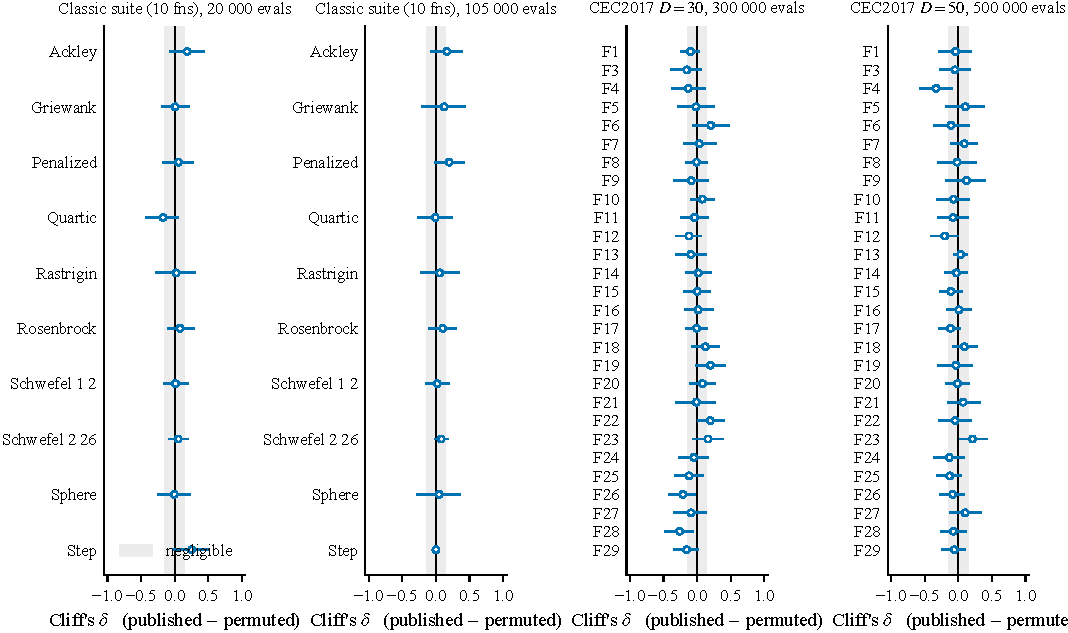
\includegraphics[width=\textwidth]{fig_placebo_forest}
\caption{Published method against its permutation control, per function, with
bootstrap intervals. Shading marks the negligible band $|\delta|<0.147$.}
\label{fig:supp:forest}
\end{figure*}

\section{Equivalence Testing, Per Function}
\label{sec:supp:tost}

A difference test can only fail to reject; equivalence has to be shown. An
interval lying wholly inside the margin establishes it, one straddling the
margin leaves the question open, and Fig.~\ref{fig:supp:equiv} makes the
distinction visible. Most intervals straddle the boundary, which is why the
main text makes its equivalence claim at suite level and, per function, only at
the small-effect margin.

Raising the run count from $30$ to the $51$ the CEC2017 protocol prescribes
narrows the median $90\%$ half-width from $0.181$ to $0.139$---exactly the
$\sqrt{30/51}$ the sampling theory predicts---and raises the count of formally
equivalent functions from $1$ to $6$ of $28$. It does not raise it further,
because equivalence at margin $m$ requires
$|\hat{\delta}|+\text{half-width}<m$ rather than $\text{half-width}<m$. With a
median $|\hat{\delta}|$ of $0.063$, the median function would need roughly
$100$ runs; on $4$ of $28$ the point estimate already exceeds $0.147$, so no
sample size places them inside that band.

\begin{figure*}[t]
\centering
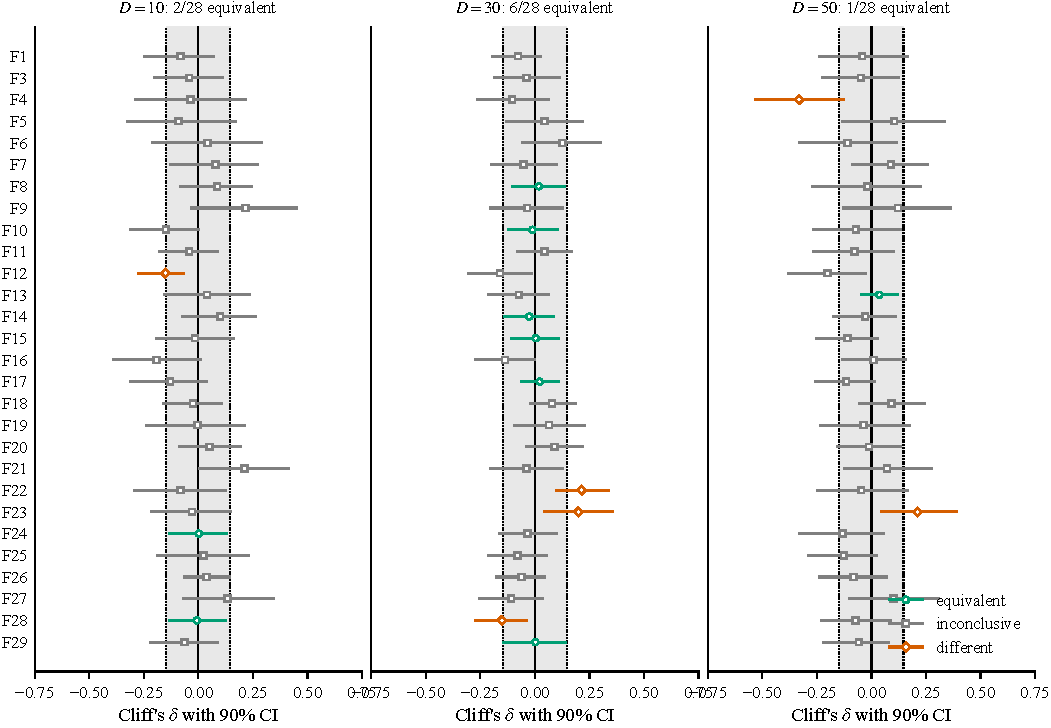
\includegraphics[width=\textwidth]{fig_equivalence}
\caption{Equivalence testing per function, published method against its
permutation control, at all three protocol dimensions. An interval contained in the shaded
margin establishes equivalence at $\alpha=0.05$.}
\label{fig:supp:equiv}
\end{figure*}

\section{Mean Ranks}
\label{sec:supp:ranks}

\begin{figure}[t]
\centering
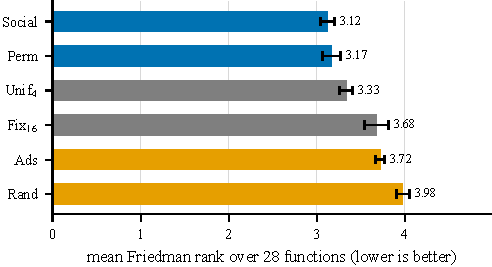
\includegraphics{fig_ranks}
\caption{Mean Friedman ranks on CEC2017 at $D=30$, with standard errors over
the $28$ functions. The published method and its permutation control are
adjacent and overlapping.}
\label{fig:supp:ranks}
\end{figure}

\section{Neighbourhood Density}
\label{sec:supp:density}

A sweep over $K\in\{4,8,16,32,59\}$ across $49$ problem configurations at their
native dimensions, $7{,}350$ runs, finds neighbourhood size to matter in $30$
of $49$ (Friedman $p<0.05$), with rank spreads up to $3.9$ of a possible $5$
and $p$ as small as $2\times10^{-23}$. Where it matters the effect is large; in
the remaining $19$ configurations it is undetectable.

Fig.~\ref{fig:supp:density} relates the preferred density to landscape
ruggedness, measured as the lag-one autocorrelation of fitness along a random
walk and therefore computable online. The association is moderate
($\rho_{s}=-0.61$, $p=3.7\times10^{-4}$), carried largely by the most rugged
functions, and it vanishes at $D=10$ ($\rho_{s}=-0.15$, $p=0.63$) while holding
at $D=30$ ($-0.73$) and $D=50$ ($-0.63$). \textsc{Penalized} and
\textsc{Penalized2} are clear counterexamples, smooth by the proxy yet
preferring the densest neighbourhood at every dimension.

\begin{figure}[t]
\centering
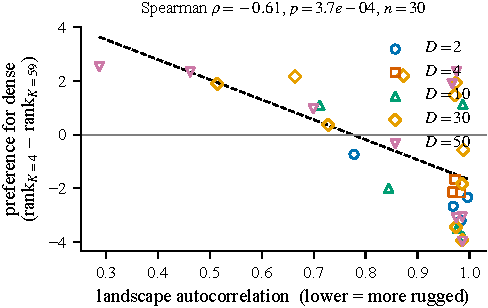
\includegraphics{fig_density_law}
\caption{Preference for dense neighbourhoods against landscape ruggedness, over
the configurations in which density has a significant effect.}
\label{fig:supp:density}
\end{figure}

\section{Implementation and Its Verification}
\label{sec:supp:impl}

The per-node update loop dominates the reference implementation's cost. We
replaced it by the sparse-matrix form of the master update, caching the
adjacency pattern and rebuilding it only when the graph is rewired. Edge swaps
preserve both edge count and degree sequence, so neither is a valid cache key;
we invalidate on an explicit rewiring counter.

Equivalence was verified before the fast path was used for any reported result.
A single diffusion step matches the reference to $8.9\times10^{-16}$ across
eight configurations---both weighting modes, both boundary-repair modes, with
and without the synchronisation step. Vectorized boundary repair matches
exactly. Over $15$ complete runs the two paths produce identical distributions
of final fitness. The speedup is $2.6\times$, bounded above by about
$3.4\times$ because the update loop is roughly $71\%$ of runtime.

\section{Hardware, Cost and Scheduling}
\label{sec:supp:hardware}

All runs execute on one machine: an Intel Core i7-12700H, $14$ cores
($6$ performance, $8$ efficiency), $32$~GB. Parallel throughput was measured
before scheduling: it saturates at about $7\times$ around $16$ workers, and
$20$ workers are slower than $16$ ($6.9\times$ against $7.1\times$) while
per-task latency nearly triples. Long batches therefore run on six worker
processes, which delivers roughly $80\%$ of peak throughput with no degradation
in per-run latency.

Parallelism uses independent sharded processes rather than a worker pool: on
this machine the pool backend fails intermittently during process spawn with a
Windows handle-duplication error. Each run checkpoints to its own file keyed by
(arm, function, dimension, seed), so sharding is equivalent to pooling,
interrupted batches resume without repeating work, and any reported number is
traceable to the run that produced it.

Cost varies by more than twentyfold across CEC2017: from $12$~s per run on the
unimodal functions to $213$~s on $F_{25}$, with composition functions averaging
$81$~s at $D=30$. Runtime estimates are therefore weighted by the suite's
actual composition rather than extrapolated from a measured rate, a
distinction that matters by a factor of three to five.

\section{Corrections to the Audited Implementation}
\label{sec:supp:corrections}

Three defects in the published implementation affect measurement and are
corrected here; we report them because they bear on the comparability of our
numbers with the original.

First, the fixed-dimension functions $F_{14}$--$F_{23}$ are evaluated at
$D=30$ although their implementations slice the first two to six coordinates,
leaving up to $28$ dimensions inert. We run each at its native dimension.
Second, neighbourhood size is set per function category, which is per-instance
tuning; we hold the population size and the schedule fixed across functions.
Third, the rewiring routine catches only \texttt{NetworkXError} while
\texttt{double\_edge\_swap} raises \texttt{NetworkXAlgorithmError}, which is
not a subclass, so dense graphs crash the optimizer; we widen the handler.

\section{Reproducibility}
\label{sec:supp:repro}

Every run is stored individually, keyed by arm, function, dimension and seed,
and every figure and table is produced by a script from those files. Seeds are
shared across arms so all comparisons are paired. The audited implementation is
published without a licence and is therefore not redistributed; the repository
carries the complete $93$-line patch against it, and the setup steps that fetch
and apply it.

\end{document}
